\documentclass[UTF8]{ctexart} % 添加中文支持

% documentclass到begin之间称为导言区,可以在这里进行一些全局设置

% 使用usepackage来添加宏包
% 所谓宏包,就是一系列控制序列的合集,这些控制序列太常用,以至于人们会觉得每次将他们写在导言区太过繁琐,于是将他们打包放在同一个文件中
% 宏包就是用于拓展Latex功能的
\usepackage{graphicx} % 用于导入外部图片的宏包(推荐格式pdf>>>>png>jpg>eps)
\usepackage{amsmath} % 使用 AMS-LaTeX 提供的数学功能
\usepackage{lmodern} % 解决字体警告问题
% \usepackage[pdf]{graphviz} % graphviz绘图支持(需要安装graphviz)
% 我的评价是还不如把latex和graphviz分开使用(latex渲染,graphviz绘图,不必非得把两者合并到一起)
\usepackage{float} % 防止图片乱浮动导致图片文字顺序混乱的包
\usepackage{multirow} % 多行表格合并的宏包
\usepackage{diagbox} % 表头斜线分割宏包
\usepackage{listings} % 代码块宏包
\usepackage{color} % 颜色宏包
\usepackage{arydshln} % 表格虚线宏包

\lstset{
    basicstyle          =   \ttfamily,          % 基本代码风格
    keywordstyle        =   \bfseries,          % 关键字风格
    commentstyle        =   \rmfamily\itshape,  % 注释的风格,斜体
    stringstyle         =   \ttfamily,  % 字符串风格
    flexiblecolumns,                % 别问为什么,加上这个
    numbers             =   left,   % 行号的位置在左边
    showspaces          =   false,  % 是否显示空格,显示了有点乱,所以不现实了
    numberstyle         =   \zihao{-5}\ttfamily,    % 行号的样式,小五号,tt等宽字体
    showstringspaces    =   false,
    captionpos          =   t,      % 这段代码的名字所呈现的位置,t指的是top上面
    frame               =   lrtb,   % 显示边框
}

\lstdefinestyle{Python}{
    language        =   Python, % 语言选Python
    basicstyle      =   \zihao{-5}\ttfamily,
    numberstyle     =   \zihao{-5}\ttfamily,
    keywordstyle    =   \color{blue},
    keywordstyle    =   [2] \color{teal},
    stringstyle     =   \color{magenta},
    commentstyle    =   \color{red}\ttfamily,
    breaklines      =   true,   % 自动换行,建议不要写太长的行
    columns         =   fixed,  % 如果不加这一句,字间距就不固定,很丑,必须加
    basewidth       =   0.5em,
}

\lstdefinestyle{c}{
    language        =   c, % 语言选Python
    basicstyle      =   \zihao{-5}\ttfamily,
    numberstyle     =   \zihao{-5}\ttfamily,
    keywordstyle    =   \color{blue},
    keywordstyle    =   [2] \color{teal},
    stringstyle     =   \color{magenta},
    commentstyle    =   \color{red}\ttfamily,
    breaklines      =   true,   % 自动换行,建议不要写太长的行
    columns         =   fixed,  % 如果不加这一句,字间距就不固定,很丑,必须加
    basewidth       =   0.5em,
}

\title{编译原理复习}
\author{Garone Lombard}
\date{\today}

\begin{document}

% 根据导言区设置生成标题、作者、日期
\maketitle % Insert the title, author and date

\newpage

\begin{abstract}
    编译原理烤漆复习手册
\end{abstract}

\newpage

% 生成目录(需要注意的是,目录的正确生成至少需要编译两次)
\tableofcontents

\newpage

\section{文法和语言}

\paragraph{文法定义} 四元组
\begin{equation}
    G=(V_T,V_N,P,S)
\end{equation}
\subsection{文法的分类}

\paragraph{0型文法} 无限制文法,只要求\emph{产生式的左部存在一个非终结符}即可。

\begin{equation}
    \forall \alpha \rightarrow \beta \in P \qquad \alpha\text{中至少包含一个}V_N
\end{equation}

\paragraph{1型文法} 上下文有关文法,在\underline{0型文法的基础上}进一步要求\emph{产生式的左部长度小于等于右部长度}
\begin{equation}
    \begin{aligned}
        \forall \alpha \rightarrow \beta \in P \qquad |\alpha| \leq |\beta| \\
        \text{产生式的一般形式}\quad \alpha1A\alpha2 \rightarrow \alpha1\beta\alpha2(\beta \neq \epsilon)
    \end{aligned}
\end{equation}

\paragraph{2型文法} 上下文无关文法(\textbf{可以描述大部分程序设计语言的文法构造}),要求\emph{产生式的左部只能是一个非终结符}

\begin{equation}
    \forall \alpha \rightarrow \beta \in P \qquad \alpha \in V_N
\end{equation}

\paragraph{3型文法} 正则文法,只有两种形式,左线性文法or右线性文法(注意是要求某一文法的所有产生式均符合左/右线性文法,而不只是P1满足左线性,P2满足右线性)。\\
正则文法和正则表达式是等价的,对于任意一个正则文法G,都存在定义同一语言的正则表达式r,反之亦然。

\begin{itemize}
    \item 左线性文法:$A\rightarrow \omega B \quad or \quad A\rightarrow \omega $
    \item 右线性文法:$A\rightarrow B \omega \quad or \quad A\rightarrow \omega $
\end{itemize}

例如
\begin{align*}
    S & \rightarrow a|b|c|d                       \\
    S & \rightarrow aT|bT|cT|dT                   \\
    T & \rightarrow a|b|c|d|0|1|2|3|4|5           \\
    T & \rightarrow aT|bT|cT|dT|0T|1T|2T|3T|4T|5T
\end{align*}

\subsection{(句型的)短语}

已知文法

\begin{align*}
    E & \rightarrow E+E    \\
    E & \rightarrow E*E    \\
    E & \rightarrow -E     \\
    E & \rightarrow (E)    \\
    E & \rightarrow idenfr \\
\end{align*}

对于句型:$-(E+E)$,可构造如下分析树

% 对于图片浮动的问题,还是得手动排版来解决
\begin{figure}[H]
    \centering
    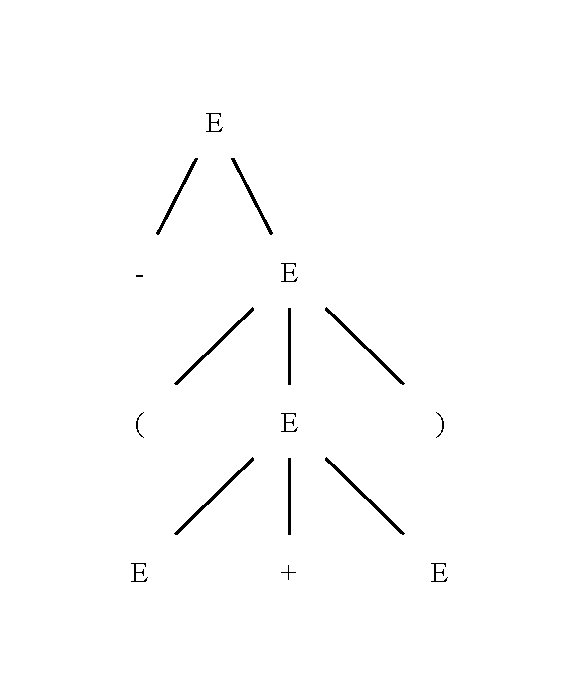
\includegraphics[width=0.7\textwidth]{assets/tree.pdf}
    \caption{分析树}
\end{figure}

\begin{itemize}
    \item $E+E$是句型$-(E+E)$相对于规则$E\rightarrow E+E$的短语,直接短语,句柄(子树层级为1)
    \item $(E+E)$是句型$-(E+E)$相对于规则$E\rightarrow (E)$的短语
    \item $-(E+E)$是句型$-(E+E)$相对于规则$E\rightarrow -E$的短语
\end{itemize}

需要注意的是,直接短语一定是某产生式的右部,但\emph{某产生式的右部不一定是\textbf{给定句型}的直接短语}

\section{词法分析}

\subsection{有穷自动机}

\paragraph{基本概念} 省略...

\begin{figure}[H]
    \centering
    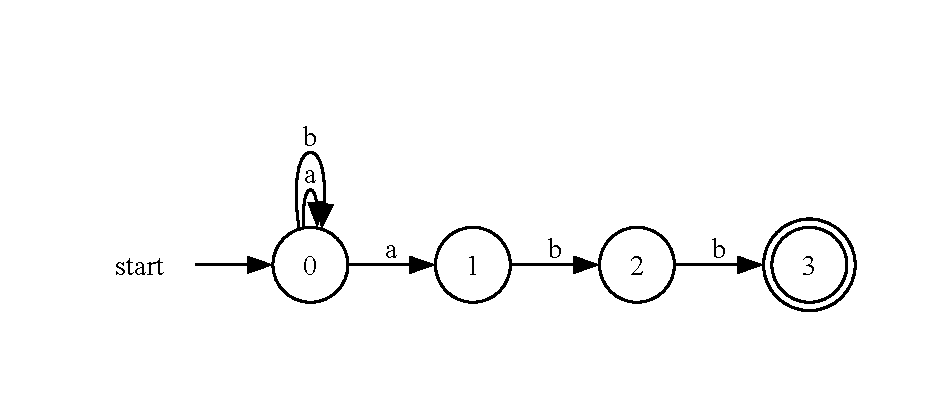
\includegraphics[width=\textwidth]{assets/FA.pdf}
    \caption{FA}
\end{figure}

\paragraph{最长前缀匹配原则} 当输入串的多个前缀与一个或多个模式匹配时,总是选择最长的前缀匹配。
也就是说在到达某个终态后,只要输入串上还有符号,FA就会继续读入下一个符号,以寻求尽可能长度的匹配。

\emph{正则表达式和有穷自动机是等价的}

\subsubsection{确定的有穷自动机(DFA)}

\paragraph{定义} DFA是一个五元组,$M=(S,\Sigma,\delta,s_0,F)$

\begin{itemize}
    \item S:有穷状态集
    \item $\Sigma$:输入符号表
    \item $\delta$:状态转移函数,$\forall s\in S,a\in \Sigma,\delta(s,a)$表示从状态s出发,沿着标记为a的边所能到达的状态(\emph{唯一})
    \item $s_0$:初始状态
    \item F:终态\textbf{集}
\end{itemize}

\begin{figure}[H]
    \centering
    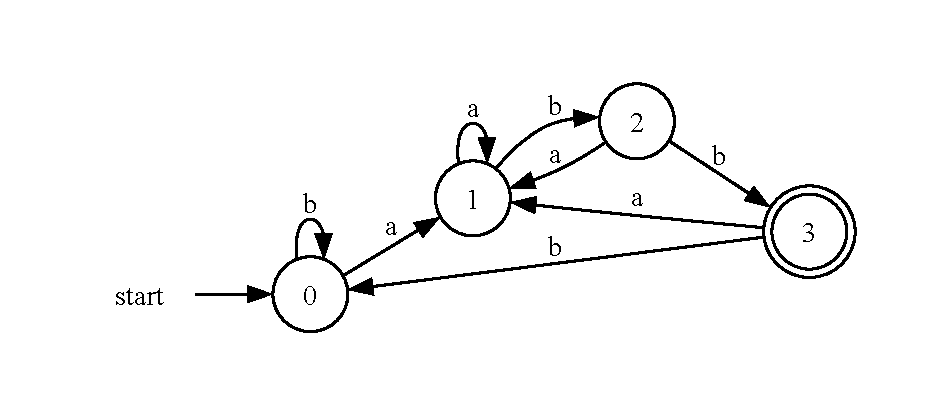
\includegraphics[width=\textwidth]{assets/DFA.pdf}
    \caption{DFA}
\end{figure}

\begin{table}[H]
    \centering
    \begin{tabular}{|p{2cm}<{\centering}|p{3cm}<{\centering}|p{3cm}<{\centering}|}
        \hline
        \diagbox{状态}{输入} & a & b \\
        \hline
        0                & 1 & 0 \\
        \hline
        1                & 1 & 2 \\
        \hline
        2                & 1 & 3 \\
        \hline
        3*               & 1 & 0 \\
        \hline
    \end{tabular}
    \caption{转换表}
\end{table}

\paragraph{DFA的算法实现}

\begin{itemize}
    \item 输入:以文件结束符eof结尾的字符串x,DFA M的开始状态$s_0$,接受状态集合F,状态转换函数$move(s,a)$
    \item 输出:M接受则输出"yes",拒绝则输出"no"
    \item 算法:
          \begin{lstlisting}[language=c,style=c]
s=s0;
c=nextChar();
while(c!=eof){
    s=move(s,c);
    c=nextChar();
}
if(s in F) output("yes");
else output("no");
          \end{lstlisting}
\end{itemize}

\subsubsection{不确定的有穷自动机(NFA)}

\paragraph{定义} NFA是一个五元组,$M=(S,\Sigma,\delta,s_0,F)$

\begin{itemize}
    \item S:有穷状态集
    \item $\Sigma$:输入符号表
    \item $\delta$:状态转移函数,$\forall s\in S,a\in \Sigma,\delta(s,a)$表示从状态s出发,沿着标记为a的边所能到达的状态\textbf{集合}
    \item $s_0$:初始状态
    \item F:终态\textbf{集}
\end{itemize}

\emph{NFA和DFA的唯一区别就是状态转换函数的状态不唯一}

\begin{figure}[H]
    \centering
    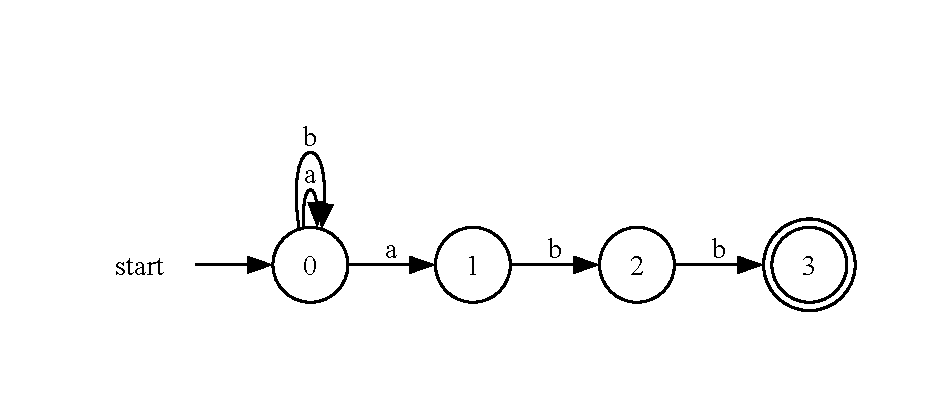
\includegraphics[width=\textwidth]{assets/NFA.pdf}
    \caption{NFA}
\end{figure}

\begin{table}[H]
    \centering
    \begin{tabular}{|p{2cm}<{\centering}|p{3cm}<{\centering}|p{3cm}<{\centering}|}
        \hline
        \diagbox{状态}{输入} & a       & b      \\
        \hline
        0                & \{0,1\} & \{0\}  \\
        \hline
        1                & $\phi$  & \{2\}  \\
        \hline
        2                & $\phi$  & \{3\}  \\
        \hline
        3*               & $\phi$  & $\phi$ \\
        \hline
    \end{tabular}
    \caption{转换表}
\end{table}

\emph{DFA和NFA具有等价性},即对于任意一个NFA,都存在一个DFA,使得两者能够识别相同的语言,反之亦然。

\paragraph{带有$\epsilon$ 转换的NFA} $\epsilon$-NFA,是一种特殊的NFA,其状态转换函数$\delta$中,$\delta(s,\epsilon)$表示从状态s出发,不读入任何输入符号,直接转移到下一个状态。

\begin{figure}[H]
    \centering
    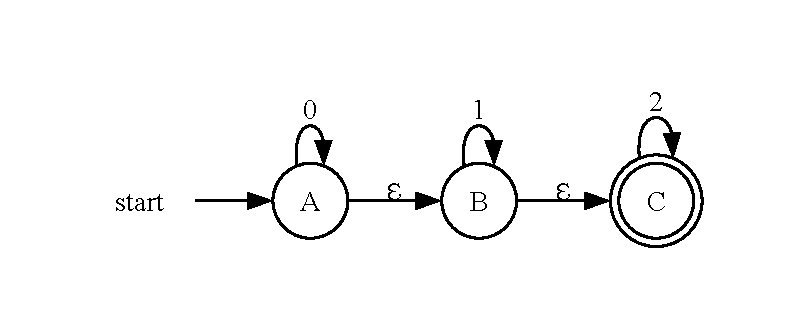
\includegraphics[width=\textwidth]{assets/epsilon-NFA.pdf}
    \caption{$\epsilon$-NFA}
\end{figure}

可以证明,对于任意一个$\epsilon$-NFA,都存在一个DFA,使得两者能够识别相同的语言,反之亦然。

也就是说,\emph{DFA、NFA、$\epsilon$-NFA都具有等价性}。

\subsubsection{从正则表达式到DFA的转换}

直接将正则表达式转换为DFA相当困难,所以一般采取$RE->NFA->DFA$的形式

\paragraph{正则表达式到NFA的转换} 对应关系如下

\begin{itemize}
    \item $\epsilon$对应的NFA
          \begin{figure}[H]
              \centering
              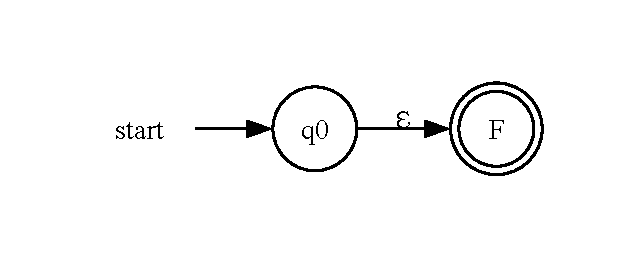
\includegraphics[width=0.7\textwidth]{assets/空串NFA.pdf}
          \end{figure}
    \item 字母表$\Sigma$中符号a对应的NFA
          \begin{figure}[H]
              \centering
              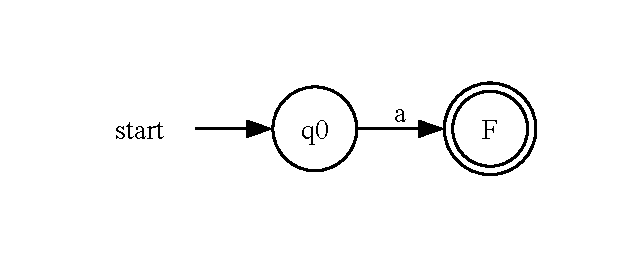
\includegraphics[width=0.7\textwidth]{assets/aNFA.pdf}
          \end{figure}
    \item $r=r_1r_2$对应的NFA
          \begin{figure}[H]
              \centering
              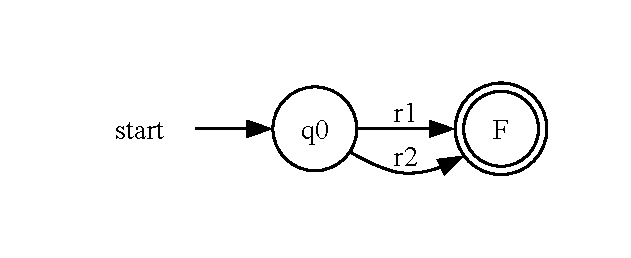
\includegraphics[width=0.7\textwidth]{assets/r1orr2NFA.pdf}
          \end{figure}
    \item $r=(r_1)*$对应的NFA
          \begin{figure}[H]
              \centering
              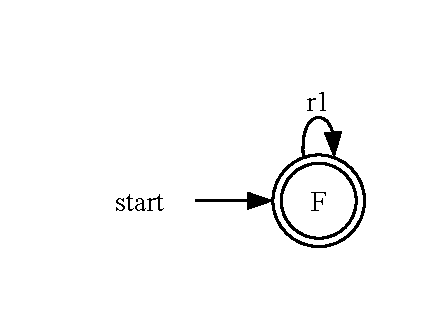
\includegraphics[width=0.7\textwidth]{assets/r1NFA.pdf}
          \end{figure}
    \item $r=(a|b)^*abb$对应的NFA
          \begin{figure}[H]
              \centering
              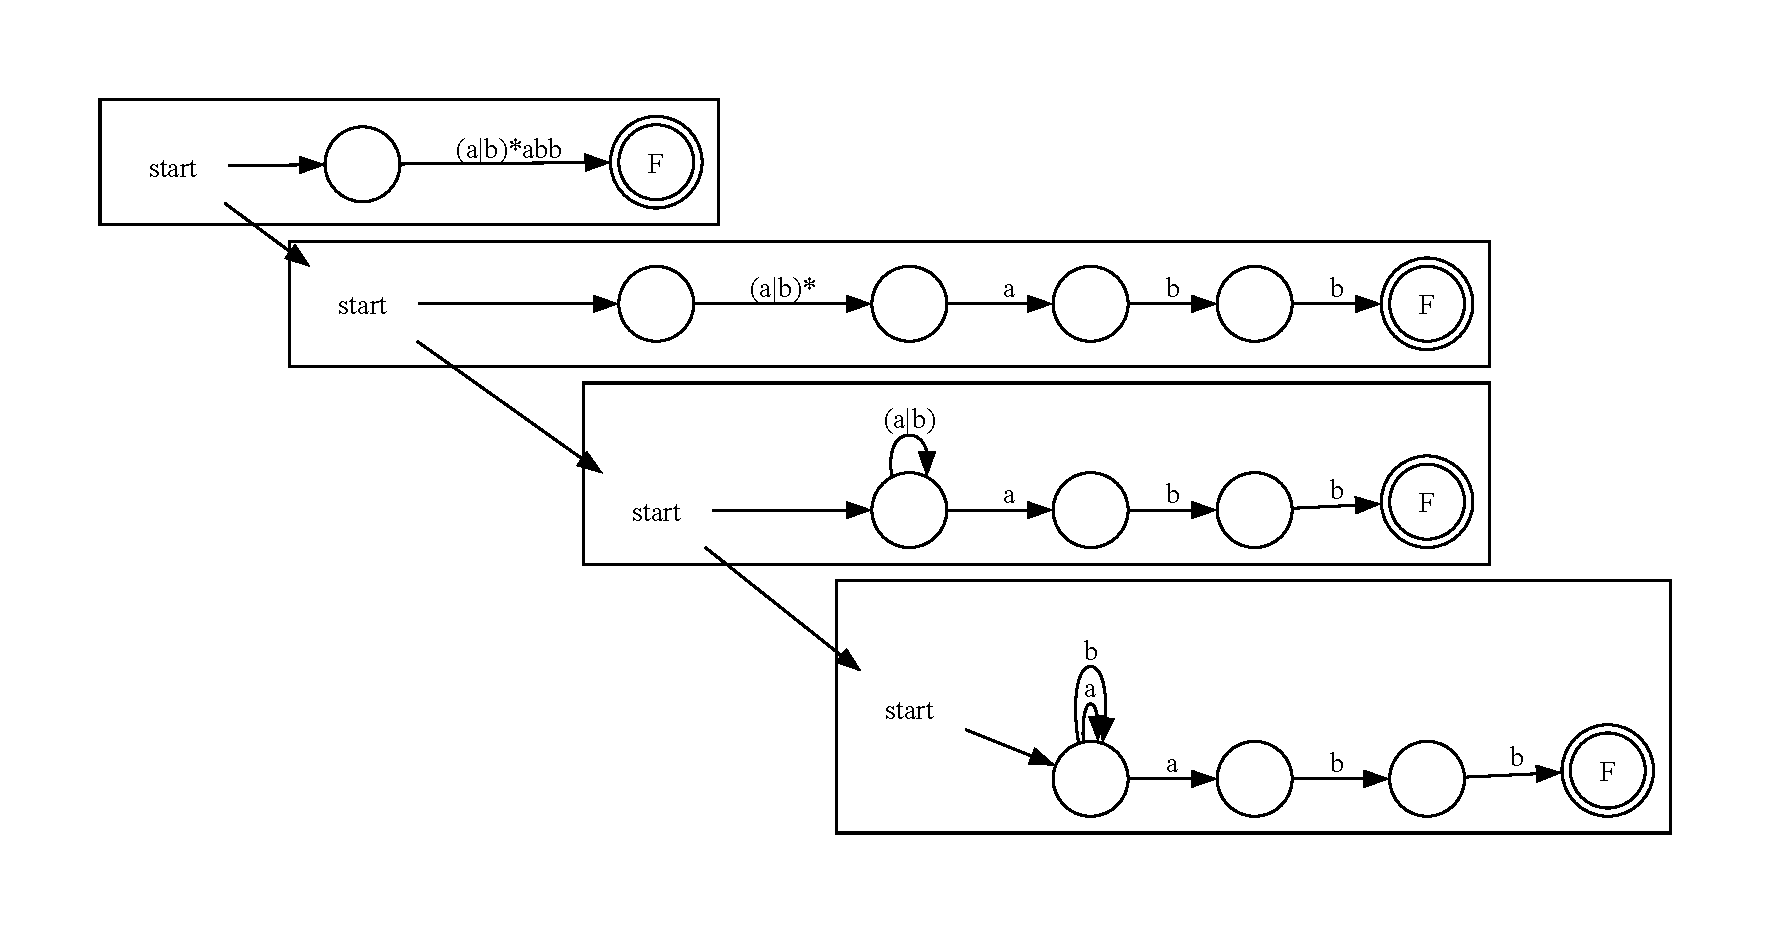
\includegraphics[width=\textwidth]{assets/ababb.pdf}
          \end{figure}
\end{itemize}

\paragraph{NFA到DFA的转换} 如下所示

\begin{figure}[H]
    \centering
    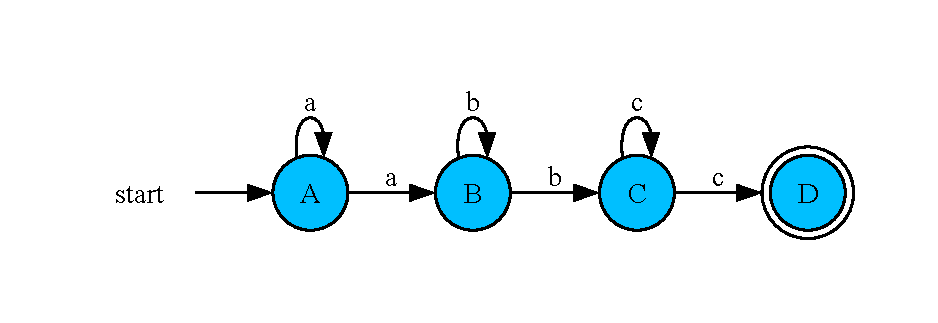
\includegraphics[width=\textwidth]{assets/nfa2.pdf}
\end{figure}

首先绘制状态转换表

\begin{table}[H]
    \centering
    \begin{tabular}{|p{2cm}<{\centering}|p{2cm}<{\centering}|p{2cm}<{\centering}|p{2cm}<{\centering}|}
        \hline
        \diagbox{状态}{输入} & a       & b       & c       \\
        \hline
        A                & \{A,B\} & $\phi$  & $\phi$  \\
        \hline
        B                & $\phi$  & \{B,C\} & $\phi$  \\
        \hline
        C                & $\phi$  & $\phi$  & \{C,D\} \\
        \hline
        D*               & $\phi$  & $\phi$  & $\phi$  \\
        \hline
    \end{tabular}
    \caption{转换表}
\end{table}

与NFA等价的DFA的每一个状态都是一个由NFA状态构成的集合

\begin{figure}[H]
    \centering
    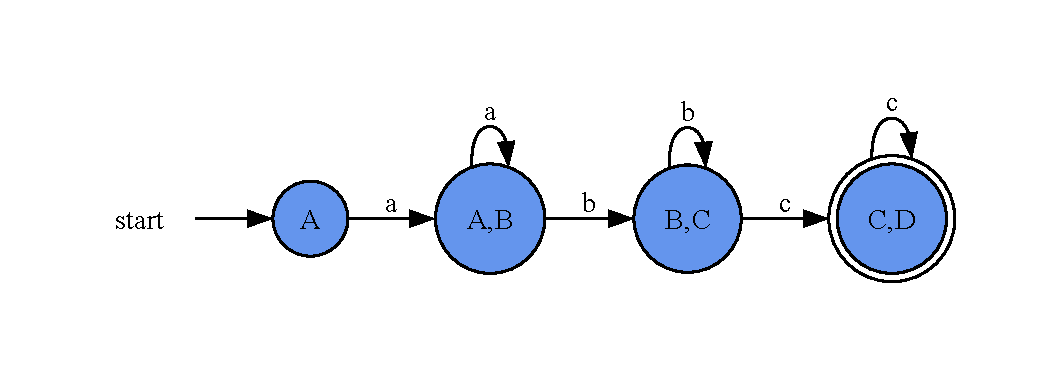
\includegraphics[width=\textwidth]{assets/dfa2.pdf}
\end{figure}

$\epsilon$-NFA到DFA的转换

\begin{figure}[H]
    \centering
    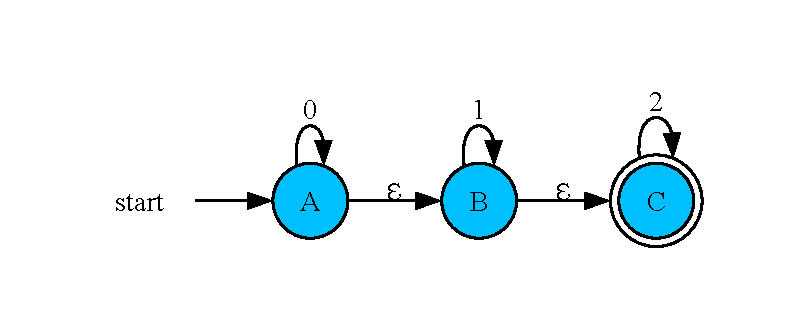
\includegraphics[width=\textwidth]{assets/nfa3.pdf}
\end{figure}

同样绘制状态转换表

\begin{table}[H]
    \centering
    \begin{tabular}{|p{2cm}<{\centering}|p{2cm}<{\centering}|p{2cm}<{\centering}|p{2cm}<{\centering}|}
        \hline
        \diagbox{状态}{输入} & 0         & 1       & 2     \\
        \hline
        A                & \{A,B,C\} & \{B,C\} & \{C\} \\
        \hline
        B                & $\phi$    & \{B,C\} & \{C\} \\
        \hline
        C*               & $\phi$    & $\phi$  & \{C\} \\
        \hline
    \end{tabular}
    \caption{转换表}
\end{table}

需要注意的是,由于初始即可达A,B,C,所以初始状态应该是{A,B,C}而不是{A}

\begin{figure}[H]
    \centering
    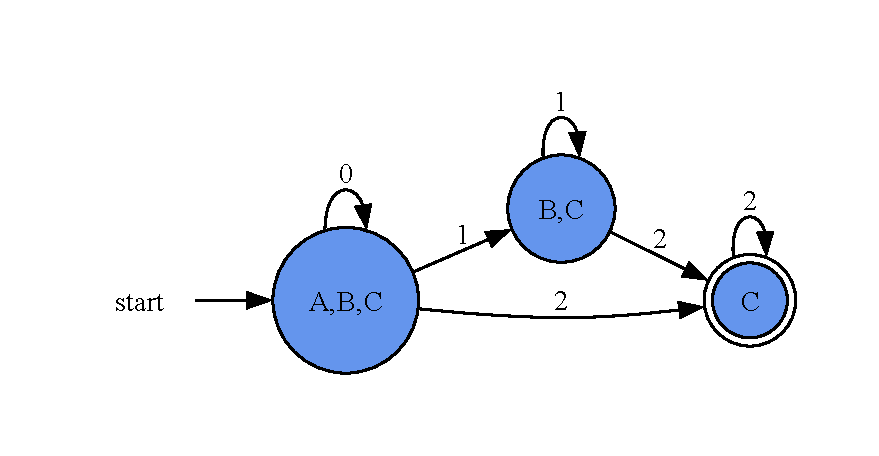
\includegraphics[width=\textwidth]{assets/dfa3.pdf}
\end{figure}

\paragraph{子集构造法}

\begin{itemize}
    \item 输入:NFA N
    \item 输出:DFA D
    \item 算法:一开始,$\epsilon-closure(s_0)$是Dstates中唯一的状态,且未加标记;
          \begin{lstlisting}[language=c,style=c]
while(在Dstates中有一个未标记状态T){
    tag(T);
    for(每个输入符号a){
        U=closure(move(T,a));
        if(U not in Dstates){
            add(Dstates,U);
        }
        Dtran[T,a]=U;
    }
}
          \end{lstlisting}
          \begin{table}[H]
              \centering
              \begin{tabular}{|p{3cm}<{\centering}|p{8cm}<{\centering}|}
                  \hline
                  操作                    & 描述                                        \\
                  \hline
                  $\epsilon-closure(s)$ & 能够从NFA的开始状态只通过$\epsilon$转换直接到达的NFA状态集合    \\
                  \hline
                  $\epsilon-closure(T)$ & 能从集合T中的某个NFA状态只通过$\epsilon$转换直接到达的NFA状态集合 \\
                  \hline
                  $move(T,a)$           & 能从集合T中的某个NFA状态通过标号为a的转换到达的NFA状态的集合        \\
                  \hline
              \end{tabular}
          \end{table}
\end{itemize}

\paragraph{NFA的化简例题} 。。。。。。

\begin{figure}[H]
    \centering
    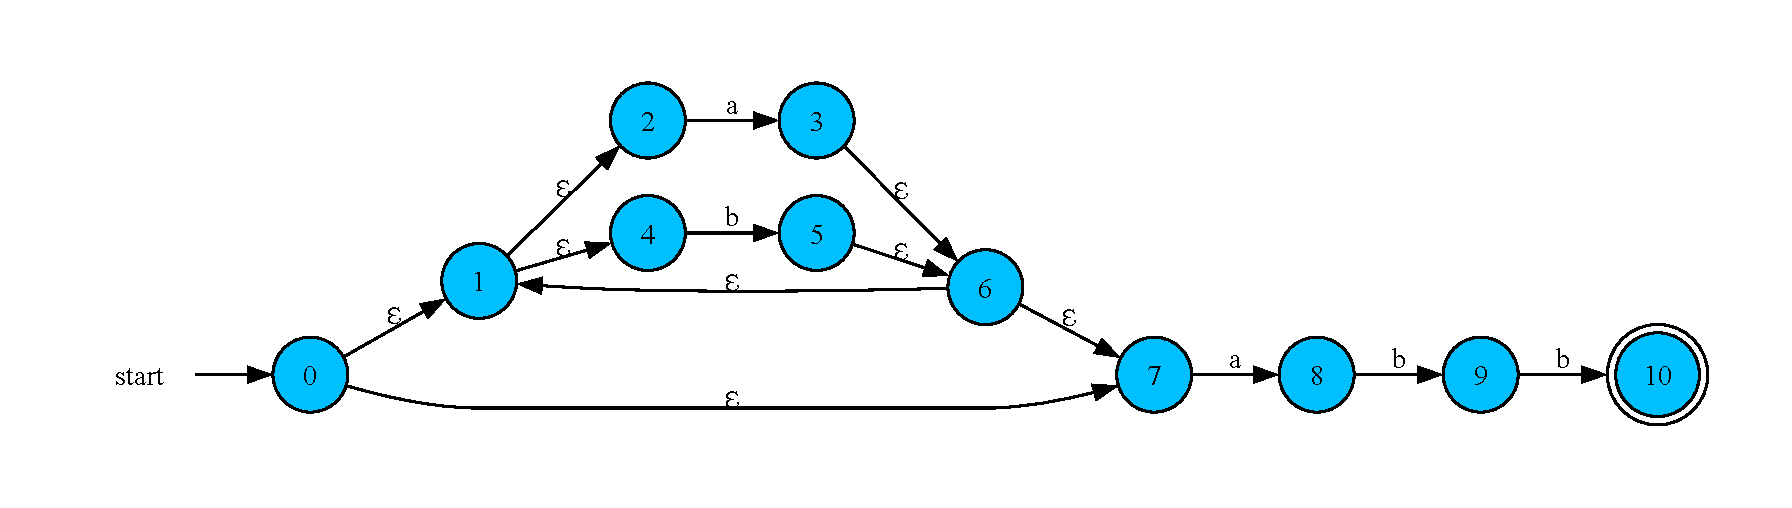
\includegraphics[width=\textwidth]{assets/nfa4.pdf}
    \caption{NFA}
\end{figure}

\begin{table}[H]
    \centering
    \begin{tabular}{|p{2cm}<{\centering}|p{3cm}<{\centering}|p{3cm}<{\centering}|}
        \hline
        \diagbox{状态}{输入} & a                 & b               \\
        \hline
        0                & \{1,2,3,4,6,7,8\} & \{1,2,4,5,6,7\} \\
        \hline
        1                & \{1,2,3,4,6,7\}   & \{1,2,4,5,6,7\} \\
        \hline
        2                & \{1,2,3,4,6,7\}   & $\phi$          \\
        \hline
        3                & \{1,2,3,4,6,7,8\} & \{1,2,4,5,6,7\} \\
        \hline
        4                & $\phi$            & \{1,2,4,5,6,7\} \\
        \hline
        5                & \{1,2,3,4,6,7,8\} & \{1,2,4,5,6,7\} \\
        \hline
        6                & \{1,2,3,4,6,7,8\} & \{1,2,4,5,6,7\} \\
        \hline
        7                & \{8\}             & $\phi$          \\
        \hline
        8                & $\phi$            & \{9\}           \\
        \hline
        9                & $\phi$            & \{10\}          \\
        \hline
        10*              & $\phi$            & $\phi$          \\
        \hline
    \end{tabular}
    \caption{转换表1(无效)}
\end{table}

\begin{table}[H]
    \centering
    \begin{tabular}{|p{3.2cm}<{\centering}|p{3cm}<{\centering}|p{3cm}<{\centering}|}
        \hline
        $\epsilon-closure(T_0)$ & \multicolumn{2}{c|}{\{0,1,2,4,7\}}                      \\
        \hline
        \diagbox{状态}{输入}        & a                                  & b                  \\
        \hline
        T0=\{0,1,2,4,7\}        & \{1,2,3,4,6,7,8\}                  & \{1,2,4,5,6,7\}    \\
        \hline
        T1=\{1,2,3,4,6,7,8\}    & \{1,2,3,4,6,7,8\}                  & \{1,2,4,5,6,7,9\}  \\
        \hline
        T2=\{1,2,4,5,6,7\}      & \{1,2,3,4,6,7,8\}                  & \{1,2,4,5,6,7\}    \\
        \hline
        T3=\{1,2,4,5,6,7,9\}    & \{1,2,3,4,6,7,8\}                  & \{1,2,4,5,6,7,10\} \\
        \hline
        T4=\{1,2,4,5,6,7,10\}   & \{1,2,3,4,6,7,8\}                  & \{1,2,4,5,6,7\}    \\
        \hline
    \end{tabular}
    \caption{转换表2(正确)}
\end{table}

\begin{table}[H]
    \centering
    \begin{tabular}{|p{3.4cm}<{\centering}|p{3cm}<{\centering}|p{3cm}<{\centering}|}
        \hline
        \diagbox{状态}{输入}       & a  & b  \\
        \hline
        T0=\{0,1,2,4,7\}       & T1 & T2 \\
        \hline
        T1=\{1,2,3,4,6,7,8\}   & T1 & T3 \\
        \hline
        T2=\{1,2,4,5,6,7\}     & T1 & T2 \\
        \hline
        T3=\{1,2,4,5,6,7,9\}   & T1 & T4 \\
        \hline
        T4*=\{1,2,4,5,6,7,10\} & T1 & T2 \\
        \hline
    \end{tabular}
    \caption{转换表2(正确)}
\end{table}

\begin{figure}[H]
    \centering
    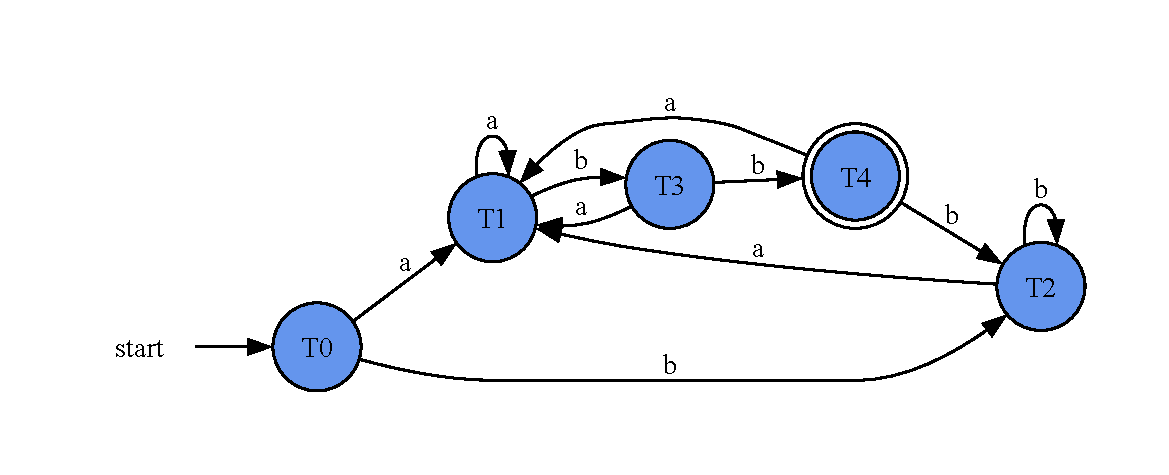
\includegraphics[width=\textwidth]{assets/dfa4.pdf}
    \caption{DFA}
\end{figure}

\subsubsection{DFA的最小化}

\paragraph{概念} 一个有穷自动机可以通过\emph{消除无用状态}和\emph{合并等价状态}来最小化

\begin{itemize}
    \item 无用状态:从该自动机的开始状态出发,任何输入串都无法到达的状态(从该状态出发,没有通路抵达终态)
    \item 等价状态:条件如下
          \begin{enumerate}
              \item \underline{一致性条件}:状态s和t必须同时为可接受状态或不可接受状态
              \item \underline{蔓延性条件}:对于所有输入符号,状态s和t必须转换到等价态
          \end{enumerate}
\end{itemize}

\paragraph{分割法} 把一个DFA(不含无用态)的状态分成一些不相交的子集,使得任何不同的两个子集的状态都是可区分的,且同一个子集中的任何状态都是等价的

\begin{figure}[H]
    \centering
    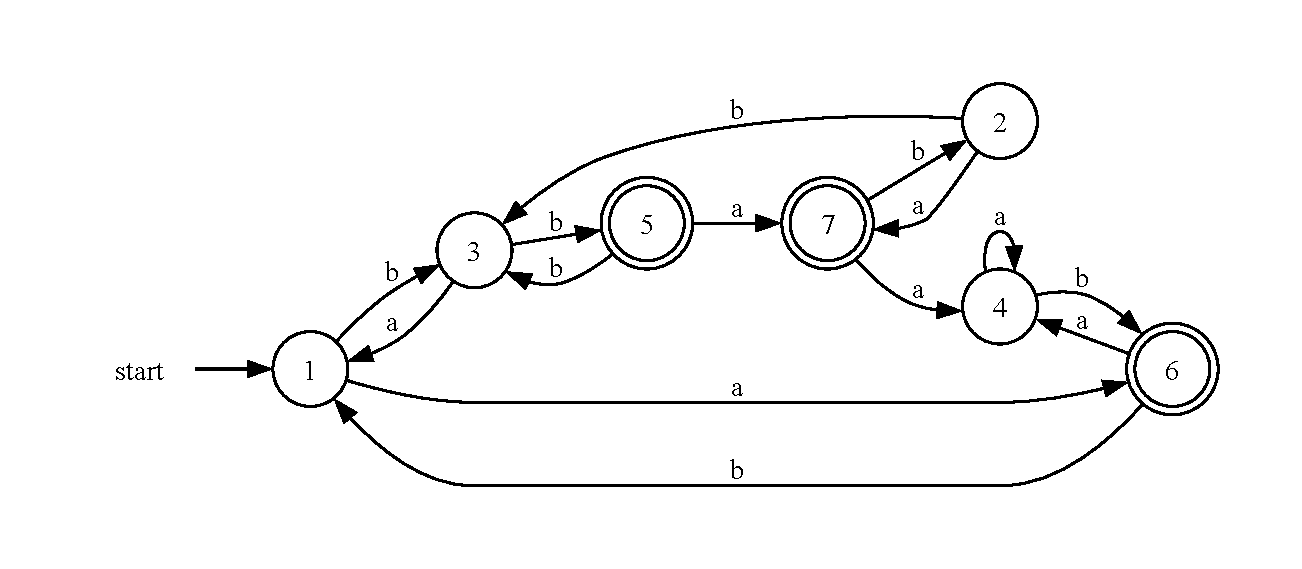
\includegraphics[width=\textwidth]{assets/dfa5.pdf}
\end{figure}

第一步都是固定的,把状态分为终态和非终态两个集合\{1,2,3,4\},\{5,6,7\}

接下来考察\{1,2,3,4\}是否可分

\begin{table}[H]
    \centering
    \begin{tabular}{|p{3cm}<{\centering}|p{2cm}<{\centering}|p{2cm}<{\centering}|}
        \hline
        \diagbox{状态}{输入} & a     & b     \\
        \hline
        1                & 6(E)  & 3(NE) \\
        \hline
        2                & 7(E)  & 3(NE) \\
        \hdashline
        3                & 1(NE) & 5(E)  \\
        \hline
        4                & 4(NE) & 6(E)  \\
        \hline
    \end{tabular}
\end{table}

因此可以将集合拆分为\{1,2\},\{3,4\},\{5,6,7\}

\begin{table}[H]
    \centering
    \begin{tabular}{|p{3cm}<{\centering}|p{2cm}<{\centering}|p{2cm}<{\centering}|}
        \hline
        \diagbox{状态}{输入} & a     & b     \\
        \hline
        1                & 6(P3) & 3(P2) \\
        \hline
        2                & 7(P3) & 3(P2) \\
        \hline
    \end{tabular}
\end{table}

显然\{1,2\}不可拆分

\begin{table}[H]
    \centering
    \begin{tabular}{|p{3cm}<{\centering}|p{2cm}<{\centering}|p{2cm}<{\centering}|}
        \hline
        \diagbox{状态}{输入} & a     & b     \\
        \hline
        3                & 1(P1) & 5(P3) \\
        \hdashline
        4                & 4(P2) & 6(P3) \\
        \hline
    \end{tabular}
\end{table}

\{3,4\}可拆分为\{3\},\{4\}

此时集合为\{1,2\},\{3\},\{4\},\{5,6,7\}

\begin{table}[H]
    \centering
    \begin{tabular}{|p{3cm}<{\centering}|p{2cm}<{\centering}|p{2cm}<{\centering}|}
        \hline
        \diagbox{状态}{输入} & a     & b     \\
        \hline
        5                & 7(P4) & 3(P2) \\
        \hdashline
        6                & 4(P3) & 1(P1) \\
        \hline
        7                & 4(P3) & 2(P1) \\
        \hline
    \end{tabular}
\end{table}

\{5,6,7\}可拆分为\{5\},\{6,7\}

因此最终得到的集合为\{1,2\},\{3\},\{4\},\{5\},\{6,7\}

\begin{table}[H]
    \centering
    \begin{tabular}{|p{3cm}<{\centering}|p{2cm}<{\centering}|p{2cm}<{\centering}|}
        \hline
        \diagbox{状态}{输入} & a     & b     \\
        \hline
        1                & 6(P5) & 3(P2) \\
        \hline
        2                & 7(P5) & 3(P2) \\
        \hdashline
        3                & 1(P1) & 5(P4) \\
        \hdashline
        4                & 4(P3) & 6(P5) \\
        \hdashline
        5                & 7(P5) & 3(P2) \\
        \hdashline
        6                & 4(P3) & 1(P1) \\
        \hline
        7                & 4(P3) & 2(P1) \\
        \hline
    \end{tabular}
\end{table}

\begin{figure}[H]
    \centering
    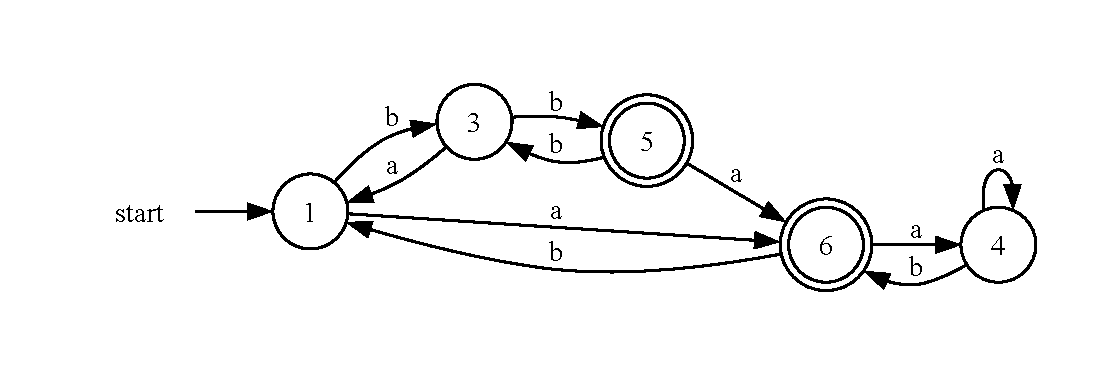
\includegraphics[width=\textwidth]{assets/dfa6.pdf}
    \caption{最小化后的DFA}
\end{figure}

\section{语法分析}

\subsection{自顶向下语法分析}

\paragraph{概念} 从分析树的顶部向底部方向构造分析树,也就是从文法开始符号S从左向右推导句子w的过程

\paragraph{最左推导} 总是选择每个句型的最左非终结符进行替换,其反过程称为最右规约

\paragraph{最右推导} 总是选择每个句型的最右非终结符进行替换,其反过程称为最左规约

在\emph{自底向上的分析}中,总是采用最左规约的方式,因此\textbf{把最左规约成为规范规约},而\textbf{把最右推导称为规范推导}

最左推导和最右推导具备唯一性,因为对于每个句型而言,其最左/右终结符是唯一的

\subsection{文法转换}

\paragraph{左递归文法} 如果一个文法中有一个非终结符A使得对某个串存在推导$A\rightarrow^{+} Aa$,那么这个文法就是左递归文法,这会使递归下降分析器陷入无限循环

处理办法如下(可消除直接左递归,其实是将其转化为了右递归)

\begin{equation}
    \begin{aligned}
        A     & \rightarrow A\alpha|\beta              \\
        A     & \rightarrow A\alpha
        \rightarrow A\alpha\alpha\alpha\alpha
        \rightarrow \beta\alpha\alpha\alpha\alpha\dots \\
        regex & =\beta\alpha^*                         \\
        A     & \rightarrow \beta A^{'}                \\
        A^{'} & \rightarrow \alpha A^{'}|\epsilon
    \end{aligned}
\end{equation}

同理,对于左递归推导$E\rightarrow E+T|T$,消除左递归可得一下等价文法

\begin{equation}
    \begin{aligned}
        E     & \rightarrow TE^{'}           \\
        E^{'} & \rightarrow +TE^{'}|\epsilon
    \end{aligned}
\end{equation}

\paragraph{$\epsilon$产生式的使用时机} 如果当前某终结符A与当前输入a不匹配时,若存在$A\rightarrow\epsilon$,可以通过检查a是否可以出现在A的后面(那不就是查看A的FOLLOW集吗?),来决定是否可以使用产生式$A\rightarrow\epsilon$

\subsubsection{FIRST集}

\paragraph{概念} 串首终结符,给定一个文法符号串a,a的FIRST(a)被定义为可以从a推导出的所有串首终结符的集合

\subsubsection{FOLLOW集}

\paragraph{概念} 可能在某个句型中紧跟在A后边的终结符a的集合

如果A是某个句型的最右符号,则将结束符\#添加到FOLLOW(A)中

\subsubsection{SELECT集}

\paragraph{概念} 产生式$A\rightarrow \beta$的可选集是指可以选用该产生式进行推导时对应的输入符号的集合,记为$SELECT(A\rightarrow \beta)$

\begin{itemize}
    \item $SELECT(A\rightarrow \alpha\beta)=\{\alpha\}$
    \item $SELECT(A\rightarrow \epsilon)=FOLLOW(A)$
\end{itemize}

如果每个具有\emph{相同左部}的各个产生式的可选集互不相交的话,就可以做出确定的分析

\subsection{自底向上语法分析}

\end{document}